\documentclass[a4paper,twoside]{article}
\usepackage{subfigure}
\usepackage{calc}
\usepackage{amssymb}
\usepackage{amstext}
\usepackage{amsmath}
\usepackage{amsthm}
\usepackage{multicol}
\usepackage{pslatex}
% added packages
\usepackage{booktabs}
\usepackage{paralist} % pour des listes en ligne
\usepackage{multirow} % pour des listes en ligne
\usepackage{varioref} % pour les références relatives
\usepackage[T1]{fontenc}
\usepackage[utf8]{inputenc}
\usepackage[english]{babel}  % gestion de la langue
\usepackage[xindy,acronym]{glossaries} % gestion des glossaire
\usepackage{natbib} % gestion de la bibliographie
\usepackage{graphicx} % gestion des images
\usepackage[super]{nth}
\usepackage{url}

\newcommand{\V}{\mathcal{V}}
\newcommand{\U}{\mathcal{U}} 

\makeglossaries
\loadglsentries{glo-csedu19}
\subfigtopskip=0pt
\subfigcapskip=0pt
\subfigbottomskip=0pt
\usepackage{SCITEPRESS} % Please add other packages that you may need BEFORE the SCITEPRESS.sty package.

\begin{document}

\title{Towards Visual Explorations of Forums' Collective Dynamics in Learning Management Systems}

%\author{\authorname{Malik Koné\sup{1,2}, Madeth May\sup{1}, Sébastien Iksal\sup{1}, Souleyman Oumtanaga\sup{2}}\affiliation{\sup{1}LIUM, Le Mans Université, Le Mans, France}\affiliation{\sup{2}LARIT, INP-HB, Yamoussoukro, Côte d'Ivoire}\email{\{malik.kone, madeth.may, sebastien.iksal\}@univ-lemans.fr, oumtana@gmail.com}}

\keywords{Visualization, Forums, Collective Learning, Learning Analytics}
\abstract{
  Discussion and exchange among peers have been hailed as an essential part of learning since at least, Vygotsky's socio-constructivist theory.  There, learning is presented as a subtle and dynamical collective process.  Hence, despite numerous efforts to understand how learners engage and maintain inspiring discussions, researchers continue to question how to reinforce effectively the collective actions.  In \glspl{lms} they propose \glspl{ldb} to learners, tutors, and managers to help them monitor various learning indicators.  But only recently have they employed  \glspl{nlp} and \gls{sna} techniques to display temporal indicators incorporating the forums' content analysis and the learners' behavioral patterns.
  In this study, we present our design efforts to model a scalable and portable indicator of collective actions.  We aim to support tutors' monitoring of forums' activities through explorable visualizations.  We review previous researches about visuals explorations of Forums' content and online collaboration's measures.  We expose in progress visualizations built from three different datasets and propose directions towards further development of indicators to monitor collective actions.
}

% on data overload (Borges & Baranauskas 2003, Dyckhoff, 2012)
% on importance interaction in forum as application of socioconstrutivsime Ferguson
% on mirroring feedback importance ?? kay 2005
% on visualization provoking understanding and self-reflexion (duvall 2011, klerkx 2014)

% TEL, LN,
\onecolumn \maketitle \normalsize \vfill

\section{Introduction}
% reseting glossary entries
\glsreset{lms}
\glsreset{ldb}
\glsreset{nlp}
\glsreset{sna}
% what's the problem ?
Modern online learning environments rely on forums and chat rooms for their students to exchange information about a subject, get help from peers and tutors or socialize.  When attendance is massive --as currently in popular \glspl{mooc}--, or if the course session spread over a long period of time, the forums' messages rapidly become intractable.  Therefore, the mass of information is devalued and can even be a burden on the learners and tutors as the former struggle to find adequate peers to support learning collectively and the latter are overwhelmed by numbers.

Efforts have been made to help tutors analyzes the students' exchanges in forums but, as we will see in section~\ref{section:3}, these analyzes are often limited to a small set of individual or are topic specific.  Also, the analysis usually takes place at the end of the learning session and does not allow ``real-time'' guidance.
% They could be improved by adding a temporal dimension and refining the semantic dimension.

Meanwhile, interactions taking place in forums account for essential aspects of the socio-constructivism learning theory.  Vygotsky emphasizes the importance of discussions as they take learners at the fringe of their knowledge domain, the proximal development zone.  There, they push back their knowledge barrier and build new knowledge to fill the gaps spotted during discussions.  Therefore, facilitating forums' usages in ways that encourage discussions and collective actions should theoretically be beneficial to the learning experience of all actors.  But as far as we know, there is yet no method to come up with a generic and dynamic way to explore the social interactions taking place in \gls{lms}.  Learners often struggle to build a sense of belonging \citep{Khalil2014} and tutors have difficulties supporting effective collective actions \citep{Zheng2015}.  The learning potential brought by the popularization of \gls{lms} is jeopardized.
%(ref bandura)
% why should one get interested in visualization of collectiv dynamics ?
Well-designed learning dashboard could help support collective actions by enabling the exploration of the forums' interactions.  They would offer the possibility for the tutor and administrator to better understand how students and discussed topics evolve, as well as facilitate the curriculum design improvements.  \glspl{ldb} could also help learners develop reflexive competencies and increase their engagement.
% (ref Zimmer)

% What benefits would be get from improving it ? or why do we need to improve it ?

In this paper, we report our first step towards facilitating collective activities with tools supporting the tutor in their visual exploration of \gls{vuci}'s forums.
% explore design guideline to build interactive visualizations showing the collective dynamics in \glspl{lms}' forums.  Our objective is to propose a method to generate these visualizations independently of the corpus and, in fine, to facilitate collective actions.
In the next section we define collective dynamic and explain why we see it differently from collaboration.  Then, in section~\ref{section:3}, we recall previous efforts made to  monitor collective actions and use \glspl{ldb} as support tools.  In section~\ref{section:4}, we present our model and propose a way to come up with an interactive visualization (or explorable) of the forum's collective dynamic.  We illustrate it, in the \ref{section:5}\sup{th}~section with our firsts visualizations built from different datasets that we will have detailed in the preceding section.  Finally, we discuss our visualizations' limitations and future developments in section~\ref{section:6}.

\section{Visualization of Collective dynamics in \glspl{lms}}
\label{section:2}
\glsreset{ldb}

The first clarification we make is between a visualization and a \gls{ldb}.  A Learning Dashboard is a ``single display that aggregates different indicators about the learner learning process and or learning context into one or multiple visualizations'' \citep{Schwendimann2017}.  We will use the term visualization when the \gls{ldb} can be made of single visualization and keep the term \gls{ldb} when it incorporates clearly several visualizations.  
We will consider discussions taking place in \glspl{lms} or in other online applications if the latest is used in an educational context.  We understand that \glspl{lms} are applications designed with the intention of being teaching tools, but sometimes we may refer to Hangout as an \gls{lms} too.   If so, it is because we consider the specific Hangouts chat from the G Suite for Education which was built with the intent to support teaching.

We collected 7 datasets from Coursera, Hangouts and Moodle.  The datasets are different in sizes and quality.  The means of collection and the dataset specificity are further detailed in Table~\ref{tab:datasets} and Section~\ref{section:4}.  

\subsection{Actions in forums}

\begin{figure}[b]
  \small{
    \caption{\label{fig:discussion}
      Illustration of how the strength of actors' ties (or links) varies as a function of time and topic overlap.  Thread 1 corresponds to actor-topic dynamic (\ref{eq:1a}) where $B$'s late post after $A$'s \nth{1} publication does not correlate strongly enough to create the link from $A$ to $B$. But $A$'s \nth{2} post is timely enough, although not exactly on the same topic as $B$'s message, to create the tie $A \dashrightarrow B$ drawn as a dashed arrow.  In thread 2, in addition to the tie $B \dashrightarrow A$, we have a topic overlap and time proximity between $C$ and $A$.  This makes a the strong tie $A \to C$.
    }}
  \centering
  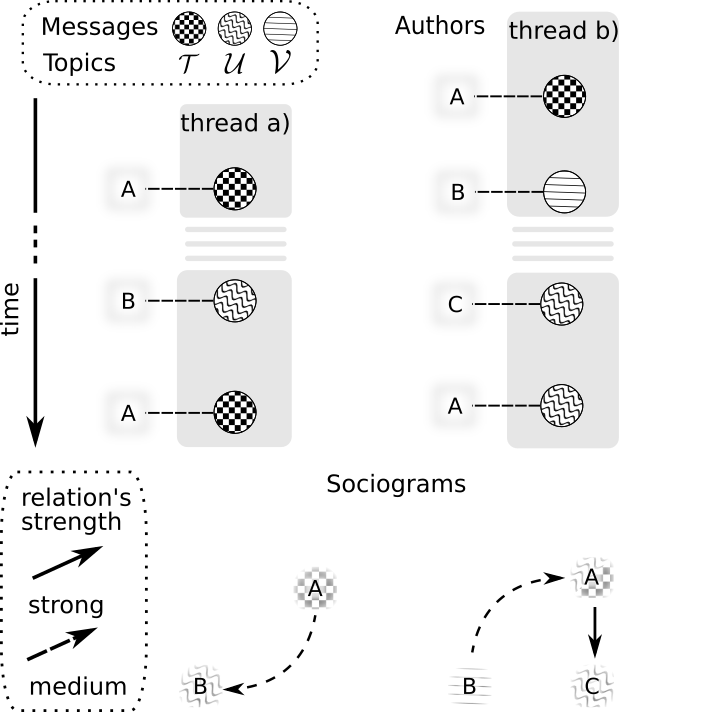
\includegraphics[width=.45\textwidth]{images/discussion.png}
\end{figure}



We make an important distinction between collaborative actions and collective actions.  \cite{Dillenbourg1999} define collaboration as a coordinated synchronous activity born from the persistent will to share a common perception of a problem originating from people with similar social roles.  It is difficult to analyze automatically collaboration if we take it as a bottom-up process with the coordination coming up from the actors themselves.  It implies that to coordinate, each actor has to evaluate the intentions of others and doing so, instantiate a theory of mind \citep{Gerstenberg2017}, which is very challenging to implement.  Therefore we use the term ``collective action'' instead of ``collaboration'' to emphasize that we do not make any assumption about the actors' intentions.  We focus on a set of observable actions and leave the deduction of the causal relationship to the observer.

The elementary actions we are most concerned with are those taking place in forum and chat rooms of \glspl{lms}.  In general, they are publications and messages' comments, but messages' up and down votes, publication times are significant and integrated in the model that we elaborate in section~\ref{section:4}.

\paragraph{Forums and Chat}

Depending on the \gls{lms}, different tools exist to facilitate discussions between peers. The main distinction is historical and separated asynchronous tools, forums, from synchronous aimed chat rooms.  Hence, forums' hierarchical structure is often more elaborated than that of chat rooms because their posts were always meant to be persistent.  On the other hand, chat rooms have better online awareness and presence indicators.

In this study, we consider that a forum is made of discussions and that each discussion is created from an initial message followed by other messages.  This sequence of messages is what we call a discussion thread.  A discussion may contain several threads if comments are allowed or if explicit references are made to previous publications.   In that case, the new thread will contain the referenced messages up to the initial one and all subsequent comments.  In chat rooms, several interrelated threads may also appear in a unique discussion when one explicitly mentions a previous message.

Despite their historical differences, today, both forum and chat room can be used for synchronous and asynchronous online discussions.  One can subscribe to a forum's discussion and receive alerts as soon as a new message is published.  On the other hand, an history of posts is kept in modern chat rooms and creation of several co-existing chat rooms has been facilitated.  Each chat room is them equivalent to a forum discussion. Finally, both forums and chat rooms display messages' timestamp and authors' information.
So for simplicity, we will call indifferently ``forum'' any virtual discussion space in a \gls{lms}.

\subsection{Collective Dynamics}

% what do you mean by collective dynamics
Collective dynamics are time-dependent interactions spurring for the messages co-occurrence in the forums' discussions.

\paragraph{Elementary dynamics}

\subparagraph{Actors' messages dynamics}
How do actors' messages spread over time ?  Let $(\tau_i)_{1, 2, 3}$ be three messages timestamp and $A$, $B$, $C$ three actors.  Collectively, the actors' messages could be distributed as $A_1, B_2,C_3$, meaning that $A$, $B$  and $C$ respectively posted one message at timestamp $\tau_1, \tau_2, \tau_3$.  But another dynamic could be that actor $A$, alone, published the three messages, thus $A_1, A_2, A_3$; or alternatively that $A$ published a message at $\tau_1$ and $B$ at timestamp $\tau_2$ and $\tau_3$, thus $A_1, B_2, B_3$.  Theses denotes different dynamics for the actors' messages.  Visualizing them helps identifying the users posting behavior and distinguishing learners' behavior, for example active and lurkers.

% ref see Medina despero, stahl 2014
% on tie strength (Granvetter 1973, Friedkin 1982)

\subparagraph{Topics' messages dynamics}
How do messages spread over time and topics ?  Or how topics are covered by messages over time ?
% Taking the previous timestamps  $(\tau_i)_{1, 2, 3}$, we could also be interested in viewing what topics were covered by messages over time.
\gls{lda} based methods are commonly used Bayesian parametric methods to approximate a message's topic or topics mixture \citep{Jelodar2017}.  To map each message to a point in topic space $\Phi$ we can also use other statistical non parametric methods such as stochastic block model \citep{Gerlach2018}.   The aim is to represent a message $M$ in the topic space which can be, for example, the set of probability distributions over $\Phi = \T\times \U \times \V$ where a point $M = (.7, .1, .2)$ denotes that the message is made of topics $\T$, $\U$ and $\V$ respectively in proportions $.7$, $.1$ and $.2$.  To simplify the next examples we suppose that each message maps to a unique topic. $M$ from topic $\T$ would be the point $(1, 0, 0)$.

A simple topic message dynamics example is  $\T_1, \T_2, \T_3$,  where all three messages are in the topic $\T$.  At the opposite we could have $\T_1, \U_2, \V_3$ where each message maps respectively to topics $\T$, $\U$ and $\V$.

This type of dynamic shows the evolution of the topics' popularity in the \gls{lms}, or the evolution of topics' interest over time.


\paragraph{actor-topics' dynamics}
How does an actor's messages cover topics over time?  Let $(A\T)_i$ be the message with timestamp $\tau_i$ posted by actor $A$ and on topic $\T$.  The two threads in Figure~\ref{fig:discussion} illustrate the following actor-topics dynamics:


\begin{subequations}
  \begin{align}
    \label{eq:1a}
    (A\T)_1, \cdots{}, (B\U)_8, (A\T)_9
  \end{align}
  \begin{align}
    \label{eq:1b}
    (A\T)_1, (B\V)_2, \cdots{},  (C\U)_8, (A\U)_9
  \end{align}
\end{subequations}

Where (\ref{eq:1a}) denotes that actor $A$ published two messages both on topics $\T$, but the \nth{2} came after $B$'s message on topic $\U$ that was published long after (${}_1,\cdots, {}_8$) $A$'s \nth{1} message.

In (\ref{eq:1b}), $B$ publishes a message on topic $\V$ immediately after $A$'s message on $\T$.  Then, after some time and other publications, $A$ posts a message on yet a \nth{3} topic $\U$, similar to what $C$ had just published on.

% We start to make a relationship between the actors' interests and the popularity of topics.

\paragraph{Compound dynamics}
From the above observable dynamics, we can define two more dynamics: the actor-actor and topic-topic dynamics.

\subparagraph{actor-actor's dynamics}

The actor-actor's dynamics can be taken as the evolution of the actor's social network where the actors are linked by message closeness and past interactions. We suppose that messages posted on overlapping topics in the same discussion by different actors potentially indicate some interactions between the authors.   This may not always be the case.

Figure~\ref{fig:discussion} exemplify how the strength of messages correlation is made of topic, temporal and actor closeness.  What is not shown in this figure is that the strength of the tie may also depend on previous actors' interactions, that is the social network built from previous messages correlations.
We will detail this in section~\ref{section:4} and explain how we avoid inferring causal interactions from the messages' correlations.

If a message is published shortly after another then their correlation should be strong.  In example~(\ref{eq:1b}), actors $A$ et $C$ would have a strong interaction because they published on the same topic $U$ and their respective messages' timestamp are close.  An interaction also exists between actors $A$ and $B$ but probably weaker because it is only based on the messages' timestamp and not the topic overlaps.  The relationship between actors $B$ and $C$ would be even weaker if it existed at all.  Their messages are far apart and not on the same topic. 

So, from the message topic, time and actor correlations we build a directed graph representing the social network of messages exchanged between the \gls{lms} actors. The evolution of that network is what we call the actor-actor dynamic.

\subparagraph{topic-topics' dynamics} This type of dynamic concerns the way topic's correlations evolves over time.  For example, if at the beginning of a course, topics $\T$ and $\U$ tend to be closely connected because students often mix them up in discussions, we hypothesize that as the course's concepts disambiguate, the relationship between the two topics will likely decrease because less and less students will publish messages mixing both topics in the same discussion.

As for the actor-actor dynamic, the topic-topic dynamic can be expressed as a temporal network (or temporal graph), but where nodes are topics and links between them represent relationships whose strength depend on a topic, time and actor' correlation.  This can be seen as a message based distance.

In thread 1 (Figure~\ref{fig:discussion}), some relation between $\T$ and $\U$ would occur for the same reason than that of $A \dashrightarrow B$.  Incidentally, the \nth{2} thread, we would have $\T  \dashrightarrow \V$ based on time proximity but also $\T \dashrightarrow \U$ based on shared author $A$.

As we will explain in the literature review, the topic-topic network may be best suited for student targeted visualization than the actor-actor network.

% Let $T_i^A$ be the message on topic $T$ by author $A$ with timestamp $\tau_i$

Finally, let's recall that for us collective dynamic is the evolution of relationships between topics and actors spurring from the messages' co-occurrences in an \gls{lms}'s forum without making an assumption about the actors' intentions.

\section{Related works}
\label{section:3}
We review previous works pertaining to collective actions and those about supporting learning with visualizations.


\begin{figure}[b]
  \small{
    \caption{\label{fig:fu}
      iForum's Dashboard \citep{Fu2017} showing (a) overall changes of post in the forum, (b) a thread representation, (c) discussions in packed forms, (d) the social network and (e) the details of a discussion.
    }}
  \centering
  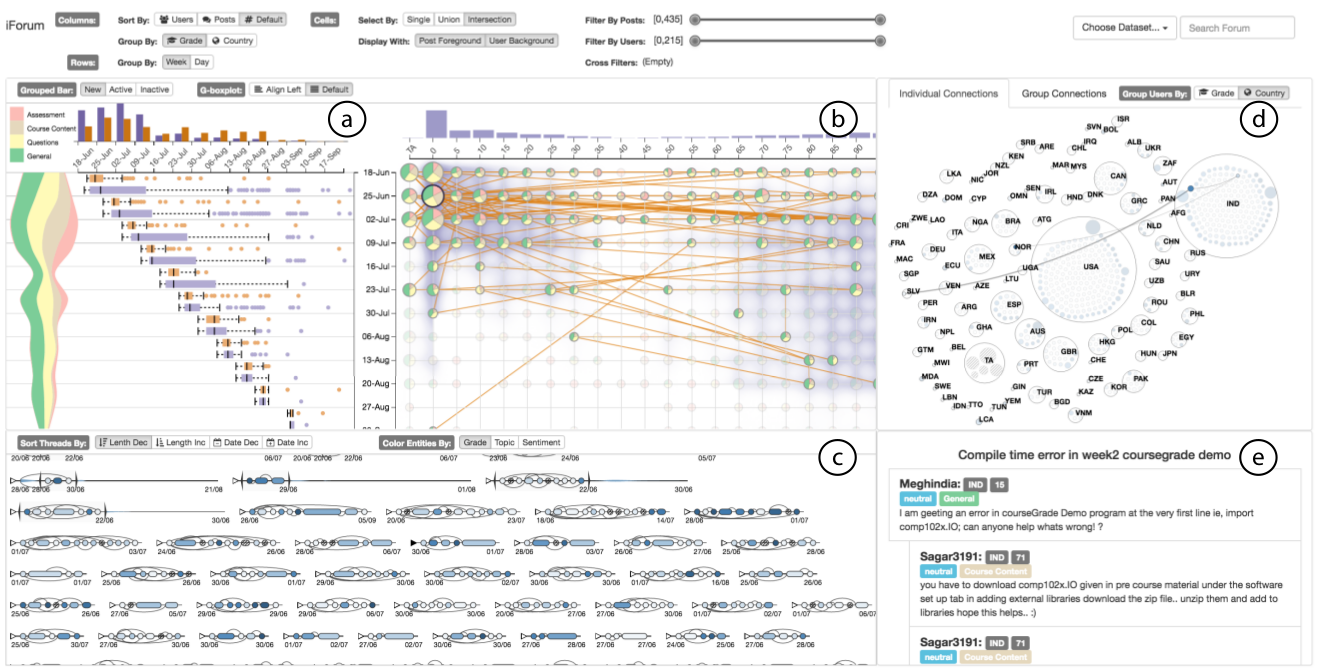
\includegraphics[width=.5\textwidth]{images/fu.png}
\end{figure}


\subsection{Analyzing collective actions}
Studies that consider collaboration usually try to identify the intentions by studying the student's behavior and the message publications.


\paragraph{Detecting collective action}  In a 250 strong \gls{col}, \cite{Rehm2015} compare on-task users, those showing engagement and high performance, with off-task users.  They use questionnaires to relate the different behaviors to the users' hierarchical position in the \gls{col}.  They compared the actors' social network position and their engagements in learning discussions.  They found a positive correlation both dimension, therefor the author did not invalidate their hypothesis that the social position influenced the learning behavior. % With \gls{sna} tools this results can tested in larger online networks.

\cite{Wang2016} are other researchers interested in the learning~of off-topic and on-topic users.  After a detailed analysis of forum messages, they demonstrate that on-topic users, that is high-order thinking users displaying constructive and interactive behaviors in the forums, have more learning gain than off-topic learners.  In conclusion, the authors advocate for an off-topic discussion detector mechanism to guide users back on more constructive grounds.

In \citep{Chua2017}, the authors' approach is to study the turn-taking in discussions.  They identify different types of conversation and categorize the users as: loner, replier, initiator without reply, initiator who respond, active social learner, active social without turn-taking, reluctant active social learners.  Beside their valuable categorization, an important result is that they observe more engagement from recurrent posters, that is poster replying to comments made to their initial posts.

If the importance of collective action for learning is agreed upon, the difficulty is identifying it at scale.  It is a complex process needing content, temporal and social network analysis.  The previous studies justify the importance of a detailed content analysis but they relied on human intervention limiting their potential to scale up.
% Only recently papers tried to tackle the problem automatically.

\paragraph{Scaling up}

\cite{Dascalu2017,Boroujeni2017} are the first big scale attempts that we found taking in account time, message content, social and dialogue structure.  Each model the students' dynamics with a mixture of \gls{nlp} techniques (bags of words, \gls{lda}, word dictionaries) and \gls{sna} (eg. block models) applied to big temporal datasets.  \cite{Dascalu2017}'s dataset contains  3,685 contributions from 179 participants and spans 2 years.  \cite{Boroujeni2017} use 2 datasets of respectively 7,699 and 12,283 messages written by 1,175 and 1,902 participants.

\cite{Dascalu2017} proxy collaboration with a Cohesion Network Analysis score applied to synchronous chat room discussions.  It correlates significantly with human discussions' analysis but it is not tested to identify collective actions as the learners were forced by pedagogical design in collaborative groups.

\cite{Boroujeni2017} analyze the influence of the course structure (timing and amount of the staffs' publications) on the forum structure, content and on the social network of learners.  They are able to show the course structure was only linked to the forum structure (number and timing of posts by students) and not to the forum content or the social network built from the forum interactions of the students.  They also report that although some learners do not publish often, they still have an important impact in forums because they sometime trigger long discussions on course's topics.  Finally, the authors recommend combining forum activity prediction model with content analysis to support instructors focusing on important discussions.

These two studies exemplify the possibility to get collective actions indicators based on content, structure and time, and as in \citep{Ezen2015} the push for better support tools for tutors.
% had previously successfully applied an unsupervised \gls{nlp} clustering technique for synchronous discussions to asynchronous one.  They conducted their experiment with final aggregated data and recognize that end users would need a real time support with a more detailed content analysis.  

\begin{figure}[t]
  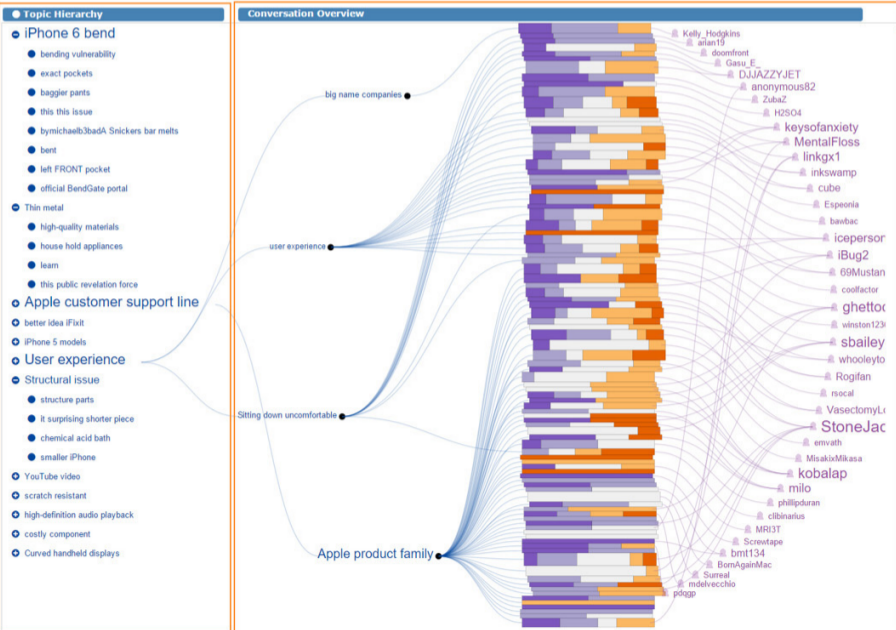
\includegraphics[width=.5\textwidth]{images/convis.png}
  \small{
    \caption{\label{fig:convis}
      Convis Dashboard \citep{Hoque2016} helps explore conversations.  On the left, the topics found in the forum using \gls{lda} and organized hierarchically.  In the middle, the colored rectangles show a sentiment analysis for each message. Each message is linked to his author place on a semi-circle and thus creating a social network. Finally, on the right, Convis display the detail of the conversation.    }}
\end{figure}

\subsection{Visualizations as support tools}

Visualization as supporting tools have been used successfully in teaching contexts. \cite{Heer2012} classify the important visualization types and \cite{Emmons2017,Leeuwen2014} advocate their generalization to support all \gls{lms} users.

\paragraph{Exploration and awareness tools}
% on importance of visualization for group dynamics
\cite{Medina2016} use a \gls{ldb} to provide quick and precise feedback with their Behavioral Awareness Mechanism.  They tackle the problem of portability and provide dynamic feedback across several platforms to 24 students working on collaborative projects.  They use communication, coordination, motivation, performance and satisfaction indicators to operationalized the collective actions.  Other studies showed how group awareness, i.e. rapid feedback about collective action, and visual narratives \citep{Yousuf2015} are beneficial to the students' engagement, even if no content analysis is done \citep{Davis2017,May2011,Medina2016}.
\cite{Davis2017} evaluated the impact a radar type visualization given to students in a two \glspl{mooc} providing them with awareness on what previous sessions learners had done at the same time of the course.  Their visualization had a positive impact on older students but it did not improve significantly the younger students' activity in the forums.

Generally, as \cite{Qu2015} note, there is a  ``need to develop both advanced data mining methods to reveal patterns from MOOC data and visualization techniques to convey the analytical results to end users and allow them to freely explore the data by themselves''.
With VisForum, \cite{Fu2017} answer  \cite{Qu2015}'s call.  VisForum  (Figure.~\ref{fig:fu}) provide a visual analytic system to interactively explore the forum of a \gls{lms}.  The complex interface helps the tutor group users and compare them to gain insights on the general forum's dynamic in terms of structure but also it terms of sentiment analysis.

Convis from \cite{Hoque2016} is an exploratory visualization that also satisfy \cite{Bull2016}'s recommendation for negotiable user models (Figure.~\ref{fig:convis}).  It is a forum exploration tool designed around a topic model that evolves with users' feedback.   It facilitates finding insightful messages from discussions
crammed with hundreds.
Finally, \cite{Guo2017} propose TieVis, an original scalable visualization specifically tailored to track explore and analyze dynamics in interpersonal links, like those we could have between the actors mentioned in the previous section.


\begin{table*}[t]
  \begin{tabular}{lllrrllp{0.14\textwidth}}
    \toprule
    \multicolumn{1}{c}{\multirow{2}{*}{Dataset}} & \multicolumn{ 1}{p{0.08\textwidth}}{\multirow{2}{*}{Discussion}} & \multicolumn{ 1}{p{0.07\textwidth}}{\multirow{2}{*}{Message}} & \multicolumn{ 1}{p{0.07\textwidth}}{\multirow{2}{*}{Author}} & \multicolumn{2}{c}{Time} & \multicolumn{ 1}{c}{\multirow{2}{*}{Structure\sup{i}}} & \multicolumn{1}{c}{\multirow{2}{*}{Extra\sup{ii}}} \\ [.1cm] \cline{ 5- 6}

    \multicolumn{ 1}{c}{source} & \multicolumn{1}{c}{(\#)} & \multicolumn{1}{c}{(\#)} & \multicolumn{1}{c}{(\#)} & \multicolumn{1}{p{0.08\textwidth}}{Span (d)} & \multicolumn{1}{r}{Precision} & \multicolumn{ 1}{l}{} & \multicolumn{ 1}{l}{} \\ \hline

    Moodle (2009) &  &  & \multicolumn{1}{l}{} & \multicolumn{1}{l}{} &  &  &  \\ [.2cm]
    FFL & \multicolumn{1}{r}{348} & \multicolumn{1}{r}{1490} & 19 & 78 &  \multicolumn{1}{l}{s} & T & Active time, Citations, Att. \\ \hline

    Coursera (2017) &  &  & \multicolumn{1}{l}{} & \multicolumn{1}{l}{} &  &  &  \\ [.2cm]
    PP & \multicolumn{1}{r}{868} & \multicolumn{1}{r}{2548} & 1112 & 365 & [1 h; 2 m]\sup{iii} &W, G \& A & V \& C \\
    PML & \multicolumn{1}{r}{1135} & \multicolumn{1}{r}{4157} & 982 & 240 & [5 h; 1 m]\sup{iii} & W, G \& A & V \& C \\
    AT & \multicolumn{1}{r}{248} & \multicolumn{1}{r}{549} & 311 & 728 & [1 d; 1 y]\sup{iii} & W \& A & V \& C \\ \hline

    Coursera (2018) &  &  & \multicolumn{1}{l}{} & \multicolumn{1}{l}{} &  &  &  \\ [.2cm]
    HR & \multicolumn{1}{r}{499} & \multicolumn{1}{r}{1004} & 638 & 989 & \multicolumn{1}{l}{ms} & W, G \& S & V, C \& Sub. \\
    UFM & \multicolumn{1}{r}{1318} & \multicolumn{1}{r}{9460} & 4609 & 1022 &  \multicolumn{1}{l}{ms} & W, G \& S & V, C \& Sub. \\ \hline

    Hangouts (2018) &  &  & \multicolumn{1}{l}{} & \multicolumn{1}{l}{} &  &  &  \\ [.2cm]
    \gls{vuci} & \multicolumn{1}{r}{5} & \multicolumn{1}{r}{7297} & 96 & 327 &  \multicolumn{1}{l}{s} & G \& S & -  \\   \bottomrule
  \end{tabular}
  \caption{\label{tab:datasets}List of datasets and courses that we use to experiment our \gls{ldb}.  \sup{i}The forum structure is given by the existence of different forum types: Weekly (W), General (G), Technical Support (S), Thematic (T) or Assignment (A) related.  \sup{ii}Extra information is often available, such as messages up votes (V), comments (C), subscription (Sub.) or attachment (Att.).  \sup{iii}When data was scrapped, the dates were in humanized format (e.g. 6 month ago, 23 minutes ago), therefore the precision varies with posts' ages.  Recent posts can be compared with greater precision than older ones. We give the intervals in which the precision varies in hours (h), days(d), month (m) and year (y).}
\end{table*}


The limit of these researches is their complex visualizations.  iForum required an extensive explanation from the designers to help the instructor grasp what was shown.  Similarly, in Convis some users reported difficulties to use the visualization efficiently and in TieVis the authors recognized that some of their visualizations were not intuitive at all.

It is clear that visualizations can help creativity and holistic thinking; improve the ability to make effective inferences; that translating or making visual analogies reinforces conceptual development; impacts cognition, helps sense-making and understanding \citep{Klerkx2014}.  \cite{Twissell2014} although in agreement with \cite{Klerkx2014} clarify the visualizations limits : 
\begin{inparaenum}[\itshape a\upshape)]
\item different learning styles, natural differences in learners have a significant impact on the way diagrams are perceived, visualized and understood
\item visualizations do not equally affect all types of learning activities.
\end{inparaenum}


\paragraph{Visualizations' effectiveness}

The study from \cite{Anaya2016} investigate how to reinforce student collective actions in the \gls{lms} dotLRN.  Noticeably they focus on directly helping the students, by designing a comprehensible tree-based visualization explaining to the student why they received a recommendation to act more collectively and how having a higher-order thinking behavior would be beneficial to them.
The engineer students working on a collaborative project reported to understand the tool and generally found it useful.

Nevertheless, precaution has to be taken with visualizations for young learners because, for the least, \cite{Lonn2015} found that a \gls{ldb} could have undesired side effects on teenagers.  Analyzing students in a summer camps remedial program, they reported that an extensive usage of a \gls{ldb} down graded some mastery goal willing students to students only willing to show proof of competence.  The opposite was not witnessed.  Therefore, some students abandoned their initial motivation to understand to only care about tricking the system so that the \gls{ldb} showed that they understood.

This last experiment justifies that although we aim to support tutors with explorable visualizations, we will consider topic based visualizations rather than user-based ones.  Topic-based visualizations do not emphases individual actions and, therefore, should damper the motivations to trick the system by adopting a superficial behavior.


\section{Explorable collective dynamics model}
\label{section:4}
In this section we detail our datasets and present the model we are going to use to analyze the collective dynamics from them.
% our firsts visualizations for exploring collective dynamics.

\subsection{Dataset collection}
Table~\ref{tab:datasets} lists our seven datasets collected between 2017 and 2018.  They are organized in four groups based the datasets' origins.
The datasets contain forum information from the following online courses:
\begin{itemize}
\item Coursera (2018), a database extraction for a Human Right (HR) and Understanding Financial Markets (UFM) courses.
\item Moodle (2009), a database extraction without message content for a French as Foreign Language (FFL) course.
\item Hangouts (2018), a JSON export from the \gls{vuci}'s G Suite for Education.  It has the data from 5 chat rooms setup-up by university staff for the staffs or the students.
\item Coursera (2017), a saving of online courses using selenium web scrapper.  The dataset is then transformed and stored as a CSV file to be processed by a Python engine. It has messages' content but approximates the timestamp.  Three courses are available: Python Plotting (PP), Python Machine Learning (PML) and African Towns (AT) an urban planning course.
\end{itemize}

\subsection{Collective dynamic model}

\paragraph{Implicit relationship's strength}
Figure~\ref{fig:discussion} gives a first example of messages' correlation, or closeness, translated as interaction's strengths between their authors.  In that example, the strength is either high, low or null.  In practice the strength $s$, that we will refer to as \emph{implicit relationship's strength}, or could be anything in $[0;1]$.
We propose to define the relationship strength between two messages as a function of time, topics and actors.  This translates the idea that the messages relationship depends on :
\begin{description}
\item[{Who}] wrote them.  Do the messages' authors have already interacted together before ?  Is the author a super poster, a lonely lurker ? One will probably consider a message differently depending on his relationship to the message's author.
\item[{Time}] Obviously the delay (or time delta) between two messages influences the strength of their relationship.  But keeping that fixed, the time of posting may also have an impact on the relationship's strength.  For example, the same messages posted by the same people may be linked differently, if the first message was posted at 11~pm and the second at 6~am (time delta 7h) or if the first was posted at 8~am and the second à 3~pm (same time delta).  Although the influence of the publishing time will diminish as time delta gets larger.  If you and your friend exchange letters every 6 months, it probably does not matter if that happens in July and January or in March and September.
\item[{Content}] should also play an import role in the way messages relate to one another.  The difficulty is to reliably automate content analysis, but \gls{nlp} techniques exist to advance in that direction.
  
\end{description}
\begin{figure}[b]
  \small{
    \caption{\label{fig:func} Graphical proposition for the function  $I(s,r)$ of the messages' interaction strength. $s$ is the ``internal'' strength of two messages based on content, time and social network structure.  $r$ is ``external'' requirement, it is a parameter set by the observer.
    }}
  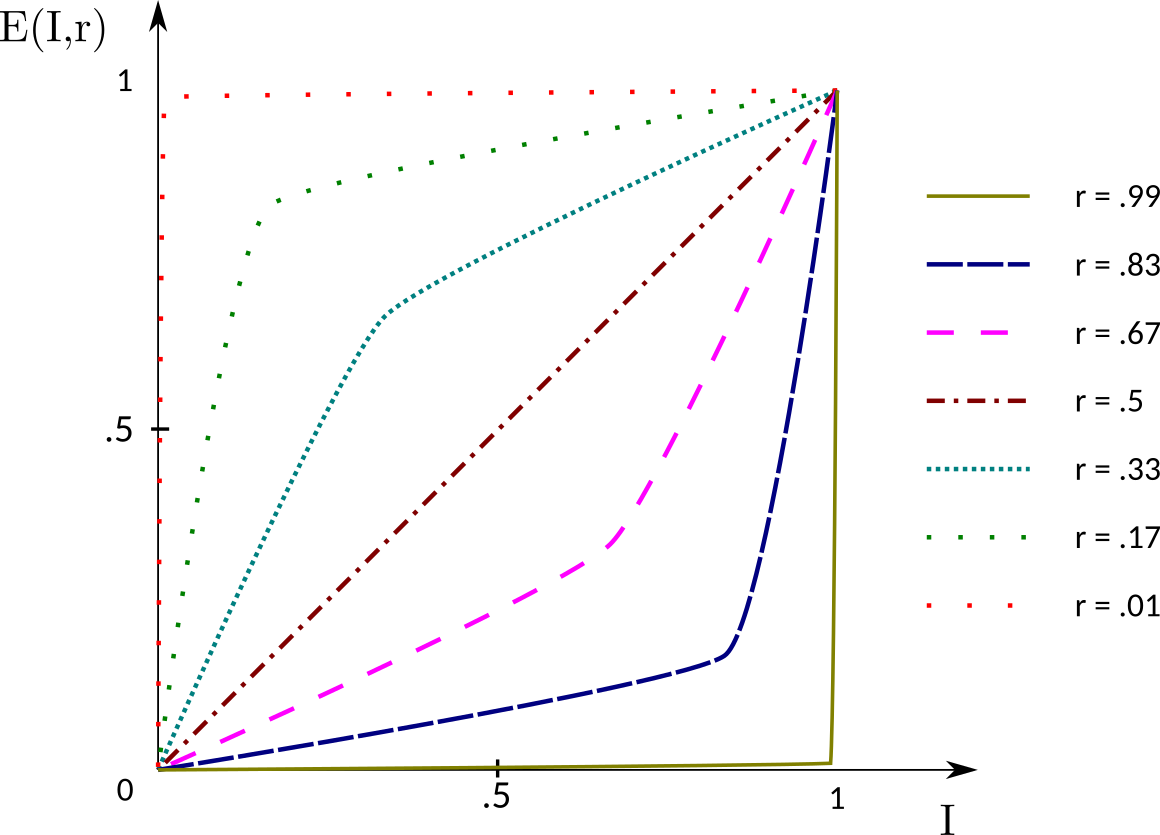
\includegraphics[width=.5\textwidth]{images/func.png}
\end{figure}

\paragraph{Required message correlation}

As we said earlier, deducting the causal relationship between messages is difficult because one has to guess what is the real intention of message's author.  To avoid making spurious deduction, we propose to make the relationship strength dependent on a parameter set interactively by the observer.  We call it the \emph{required message correlation} $r$ ($r\in[0;1]$).  If the observer set $r \approx 0$ then, for him, the requirement for a message to be linked to other messages is weak and interactions between messages, actors and topics will be common.  Although that would probably lead to overly complex and unusable dynamics metrics and visualizations.  Conversely, if $r\approx 1$, the requirement is high, meaning that the observer wants linked messages to be close in time, have a lot of topic overlap and be written from closely connected authors.  In that case messages, actor and topics will hardly have any relations with one another and dynamic will probably be invisible.

\begin{figure}[t]
  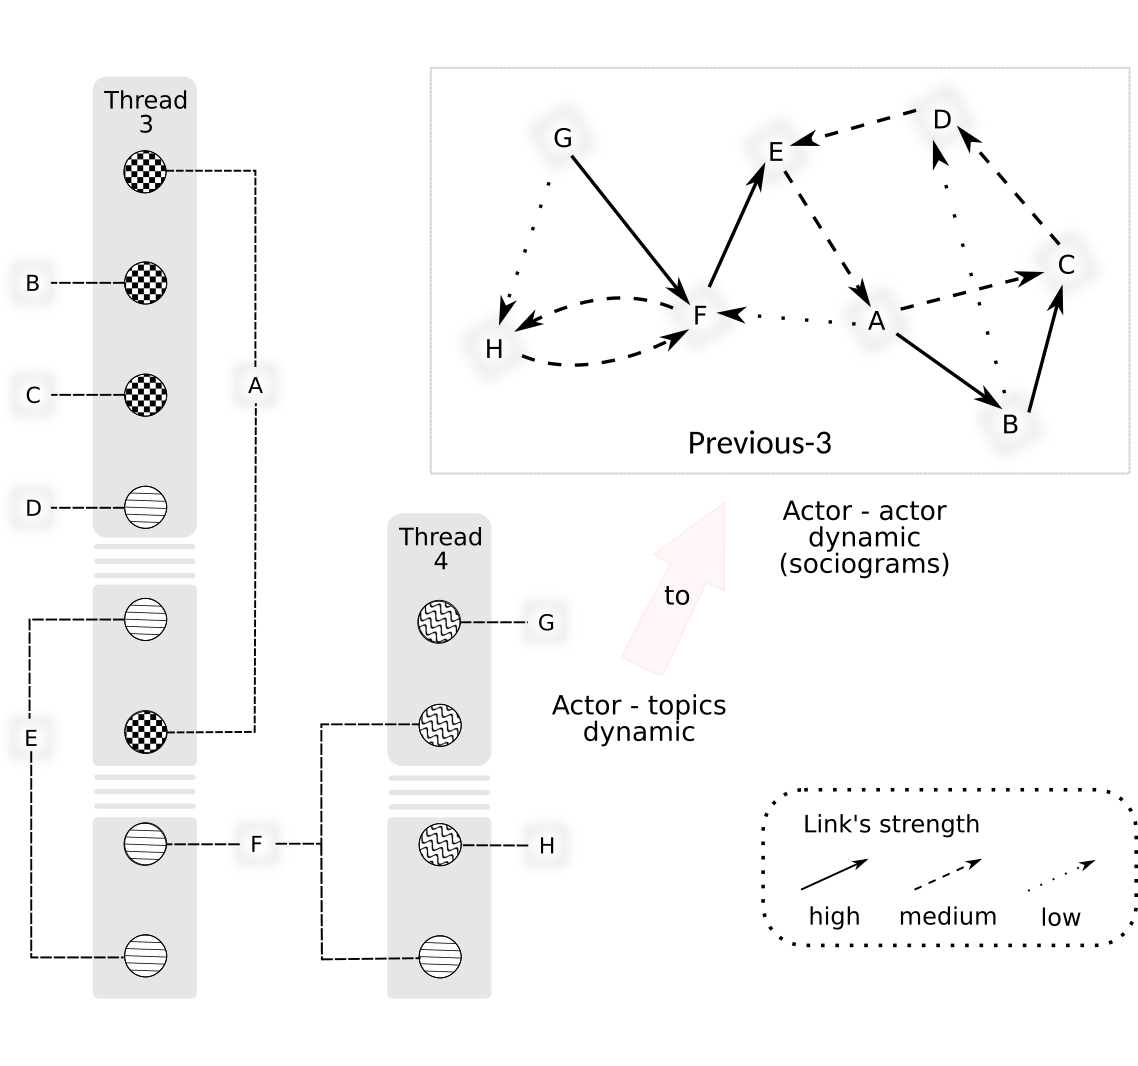
\includegraphics[width=.5\textwidth]{images/cycles.png}
  \small{
    \caption{\label{fig:cycles}
      Interactions cycles built from a bi-party actor-topic graph  Thread 3 and 4 are transformed to an actor-actor graph.  Dotted arrows denotes weaker links.
    }}
\end{figure}
 

\paragraph{Explicit relationship's strength}

% We define the causal interaction's strength $I$ between two messages as the measure of interaction taking in account the intention of the exchange.  It is a function of $s$ and $r$, where $s$ is the implicit relationship's strength, independent of the intention.  It is based on topic, time and actor closeness. And $r$ is the required message correlation, defined by as the observer's evaluation of how much implicit relationship is required to explicit it.  For all $s \in ]0;1[ $, $I$ should satisfy:
% $\lim\limits_{r \to 0} I(s,r) = 1$ and $\lim\limits_{r \to 1} I(s,r) = 0$.

% \begin{align*}
%  \lim\limits_{r \to 0} I(s',r) = 1  \qquad \text{and} \qquad \lim\limits_{r \to 1} I(s',r) = 0
% \end{align*}

% \begin{align*}
%   \forall \quad s' \in ]0;1[, \quad \left \{
%   \begin{aligned}
%     &\lim\limits_{r \to 0} I(s',r) = 1 \\
%     &\lim\limits_{r \to 1} I(s',r) = 0
%       \end{aligned}  \right .
% \end{align*}

The graph of the function $I$ could be like the one pictured in Figure~\ref{fig:func}.  If the observer's requirement is high, $r\approx{} 1$, then, for most $s$, the interaction $I$ should be low, and conversely if the observer's requirement is low, $r\approx{} 0$, then the interaction $I$ should be high, for most $s$.

We care about this interaction because it's based on its value that we display the actor-actor or topic-topic dynamics.  To further illustrate our intent, we complete our first example with longer threads (Figure~\ref{fig:cycles}).  We set four strengths to $s$: high, medium, low or $\approx 0$.  Each time or topic delta, decreases the implicit strength by one unit.  Therefore, in our case,  keeping the topic unchanged, the maximum number of relations a messages can have with ``previous'' messages is 3.  We call this connection pattern \emph{previous-3}.  But, the $s$ function could have other forms. For example, the \emph{star} pattern, i.e., $s$ been strong for the initial message but null for the others; or the \emph{previous-}$\infty$ pattern, also called ``total co-presence'' in \cite{Wise2017}, denoting non null correlations with all the previous messages.
In thread 3 (Figure.~\ref{fig:cycles}), not only does actor $D$ connects to actor $C$ but he also connects to actor $B$.  He potentially could have been connected to actor $A$ but in addition to their time delta of 3,  there a is topic delta dropping the strength of $s$ nearly to 0.  Hence, only an exceptionally low requirement $r$ would explicit $I\left ((A\T)_0,(D\V)_3 \right )$, the interaction between the messages of actors $A$ an $D$.   In our case, only if $D$ had published on the same topic as $A$, would their implicit relationship be high enough to gain visibility in our sociogram.

The results of these manipulations are a temporal actor-actor network and a temporal topic-topic network that can be represented by weighted oriented graphs.  Snapshots of an actor-actor network from the PP dataset is presented in Figure~\ref{fig:evolution}.

\paragraph{Identifying collective actions}

Once we built the actor-actor and topic-topic networks,  we want to identify potential collective actions.  Those are derived from the actor-actor network structure.
We make the hypothesis that collective actions need the presence of a recurrent actor, that is an actor replying to one of his replier \citep{Chua2017}.  We take it as the evidence that at least one of the actors has potentially assimilated someone else's message before acting, therefore initiating a collective action.
Structurally, recurrent actors form cycles in the sociogram.  For example, in Figure~\ref{fig:cycles}, actor $A$ who posted twice in thread 3 close the cycle $A \dashrightarrow E  \dashrightarrow  D  \dashrightarrow C \to B \to A$.  Further more, since actor $E$ is in cycle with $A$ and $F$, and $F$ with $H$, we will consider that actor $A$ and all of the above are engaged in a common collective action.  $G$ on the other side is not part of any cycle and, therefore, does not participate in a collective action.  In fact, $G$ published an message and disappeared.  We have no evidence that his message had an impact on others or others on his.  That is why we consider necessary (but not sufficient) that the recurrent interactions conditions collective action.   In that sens, we further \cite{Chua2017}'s findings that recurrent interactions are important for discussions.

\section{Firsts visualizations}
\label{section:5}

\begin{figure}[t]
  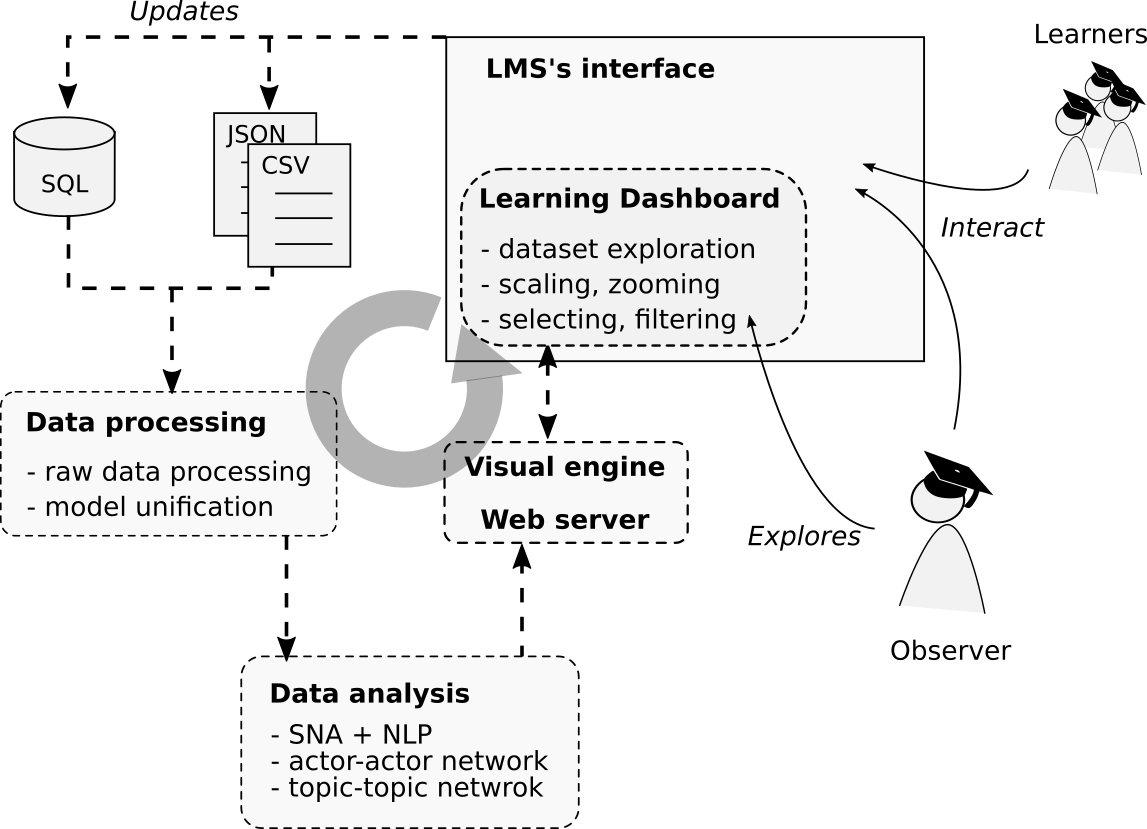
\includegraphics[width=.5\textwidth]{images/pipeline.png}
  \small{
    \caption{\label{fig:pipeline} Data Analysis cycle.
      %Regular updates or extraction from the \gls{lms} feed data repositories used processed to a unified model.  Then \gls{sna} and \gls{nlp} techniques are used to generate the actor-actor and topic-topic networks dynamics.  The visual engine use that preprocess data to generate interactive visualizations served to the \gls{lms} interface via common APIs.  Finally the observe can interact wit the visualizations and explore the topic-topic dynamics.
    }}
\end{figure}

We now introduce three visualizations from our work in progress.  They were made separately, each testing some elements of the global conception model presented in Figure~\ref{fig:pipeline}.


\begin{figure}[t]
  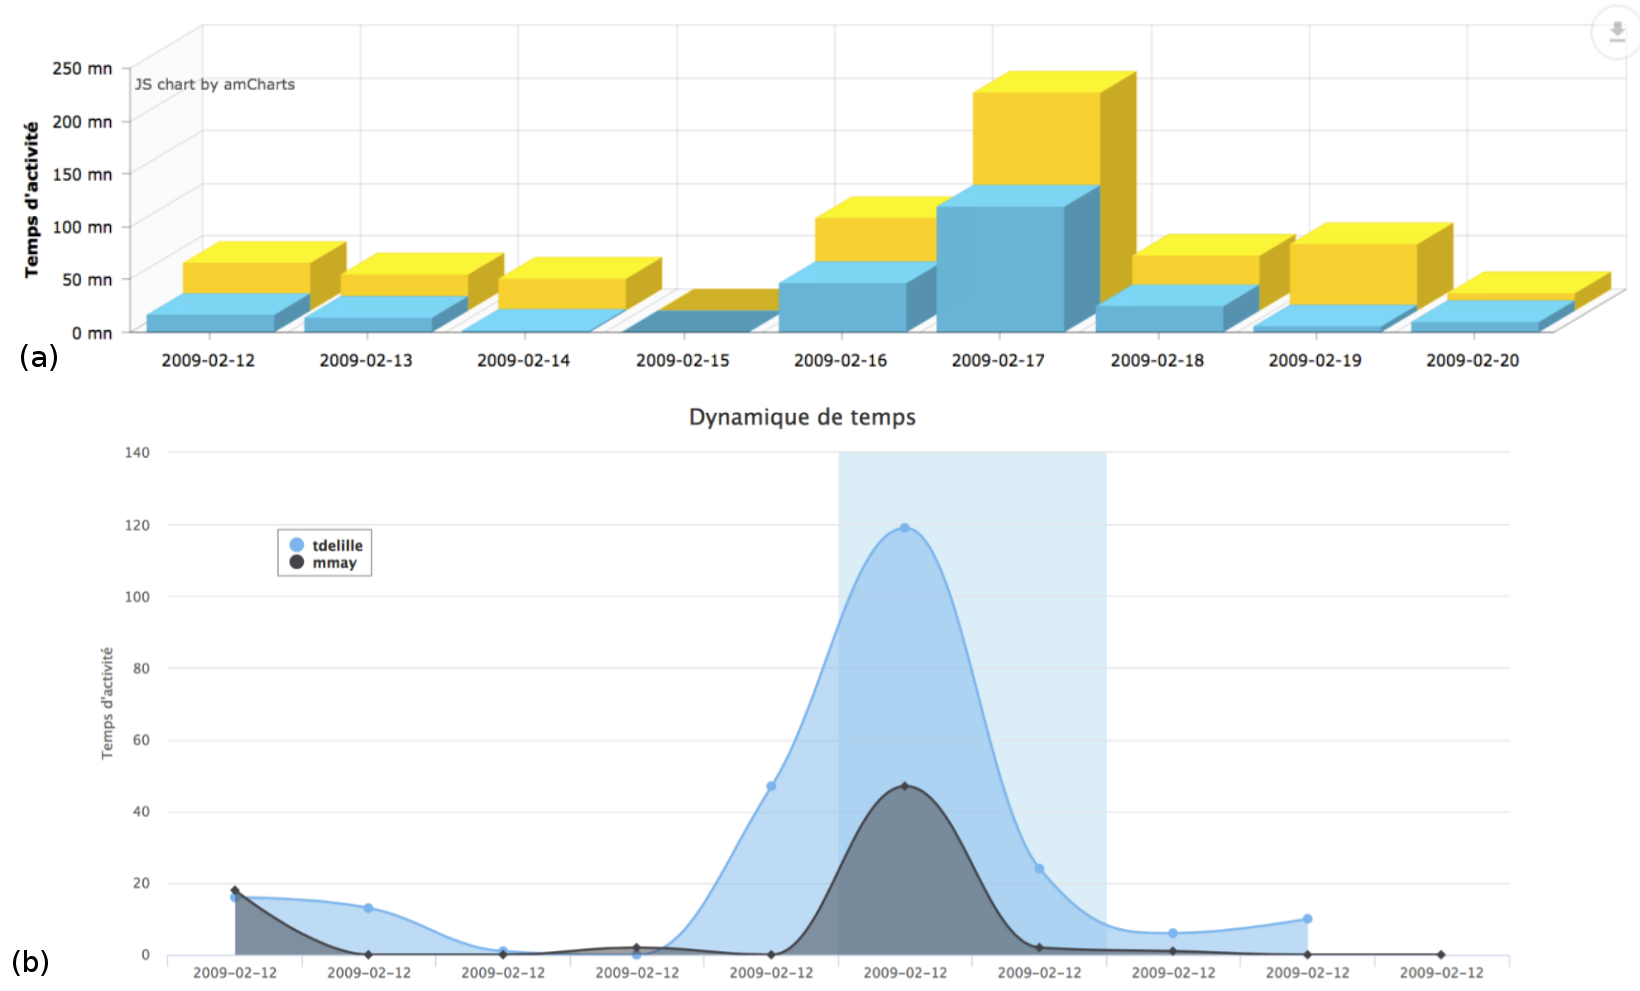
\includegraphics[width=.5\textwidth]{images/dynco_portrait.png}
  \small{
    \caption{\label{fig:dynco}
      Visualizations from the FFL dataset.
    }}
\end{figure}

\subsection{Moodle dataset}
% The work with FFL dataset tackled some issues with integrating data from a Moodle database.
We used the FFL dataset to sketch our first visualizations.  Our Moodle dataset has the particularity to contains detailed information about the actors' activity type and duration.  It enabled us to distinguish the users' active time from their idle times.  With that information we came up with the visualizations of Figure~\ref{fig:dynco}, built as part of a standalone web application.  Once we selected a user, we see the visualizations corresponding to his active time.   The top chart presents, in yellow, the total time spent in the forums for a user, day per day and compares it with his non idle activity time, shown in blue.  To handle the scaling problem, we implemented a monthly, weekly and daily based grouping criteria.  On the lower chart, we compared the activity time of two users.  We see that, although they display similar activity patterns over time, one is generally more active than the other.

This was a successful test to sketch our firsts visualizations, but the FFL dataset lacked content and its size did not create a huge monitoring problem for the tutors.  Albeit, this dataset is interesting because it emphasize the importance of the activity type.  The following step is to scale up with a bigger dataset that includes content.

\begin{figure}[t]
  \centering
  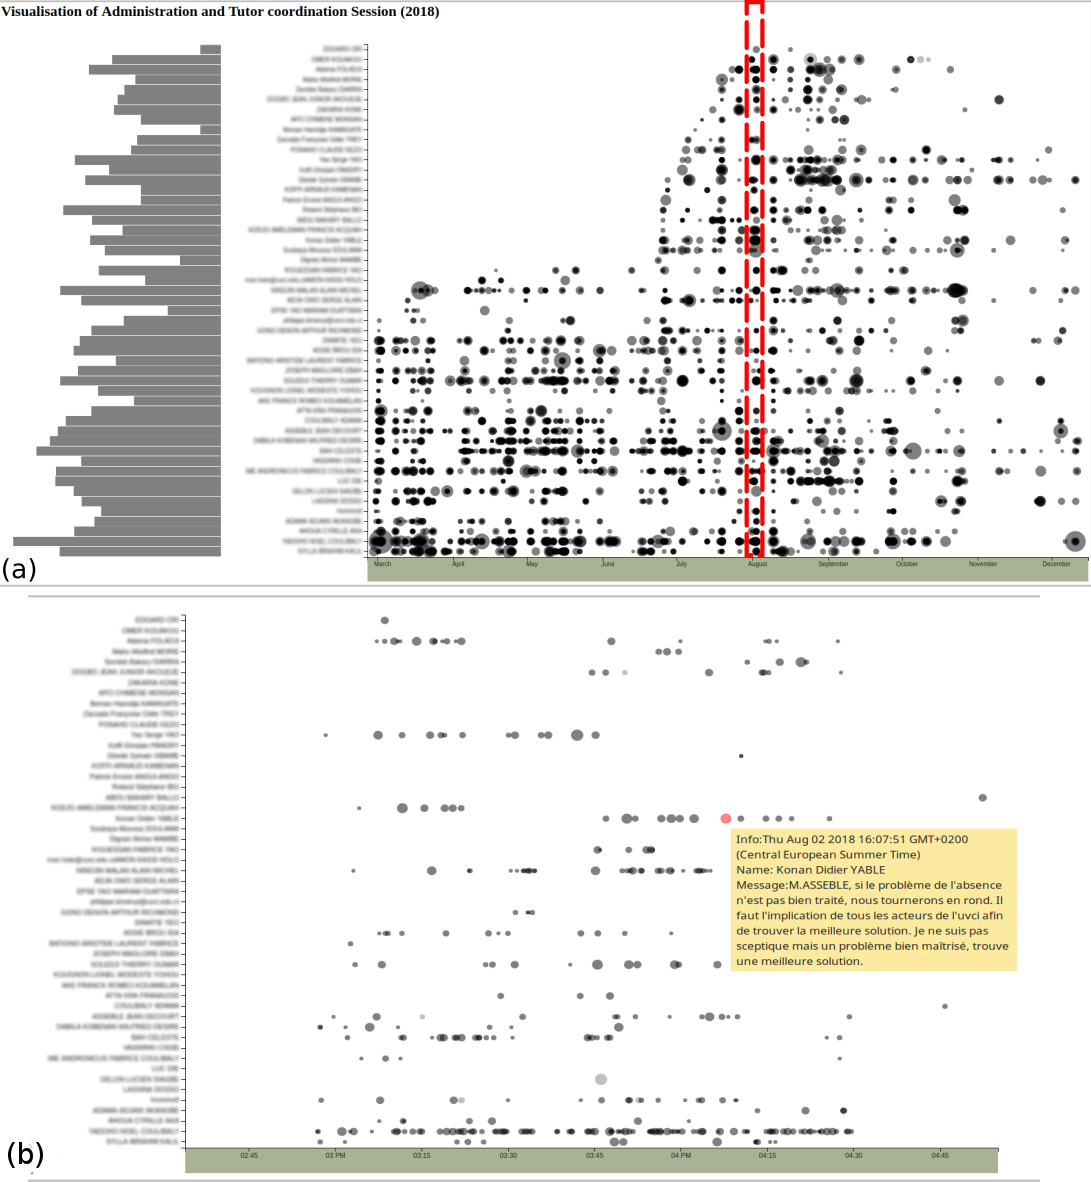
\includegraphics[width=.5\textwidth]{images/uvci_portrait}
  \small{
    \caption{\label{fig:hgconv}
      Detail of \gls{vuci} conversation taking place in 2 hours.  Each circle is a message, and hovering over them brings up its content.  The circle's size is proportional to their content's length.  Message are layered vertically by actors.  On the left is an indication of the actors total messages count.
    }}
\end{figure}

\subsection{Hangouts dataset}

The hangouts dataset is slightly different from the other datasets. It is less structured because it comes from chat rooms and not forums.  Figure~\ref{fig:hgconv} displays 6~274 messages from one chat room, gathering several threads of exchanges between the \gls{vuci}'s administration and their tutors, from March 2018 to December 2018.

We started from an manual, but automatable, export of the Google's hangouts services.  It gave us a JSON file that we preprocessed in python and fed to d3, a visualization JavaScript library, via a standalone Django web application.  We built a \gls{ldb}, testing on that larger dataset, interactive features such as zooming, panning, data point selection.
The figure's pane (a) contains a bird's eye view of all messages.  Users are represented vertically, in the middle,  with their names.  On the left is an histogram of message count for each user. On the right, along the time axis, we plotted the messages as discs whose areas are proportional to the messages' length. Activating the mouse wheel while on the time axis zoom in and out.  Bellow, is the 3 hours period framed in red, zoomed.  It shows a message pop-up, with full detail, activated by the mouse hovering a data point. 

In this investigation we did not include the \gls{sna} and \gls{nlp} analysis because our objective was the visualization of a large dataset with content and the handling of the scaling problem.  It proved that our technology choices were sound. We transformed the dataset of several thousands messages,  from the JSON file to the HTML rendering, in a few seconds.
But it also pin-pointed the importance to implement many interactive exploration functions to alleviate the scaling problem.  For examples, ways to quickly zoom on a few data points without loosing the overall picture, as well as ways to filter and order data point or axis labels, and also enabling more intricate communication between the different \gls{ldb}'s charts.
In addition to all this, a major draw back to our visualization is that it did not take in account, yet, the final users.
Finally, beside defining visual modalities, we still need to test the algorithm to compute the collective activity indicator.

\begin{figure*}[t]
  \centering
  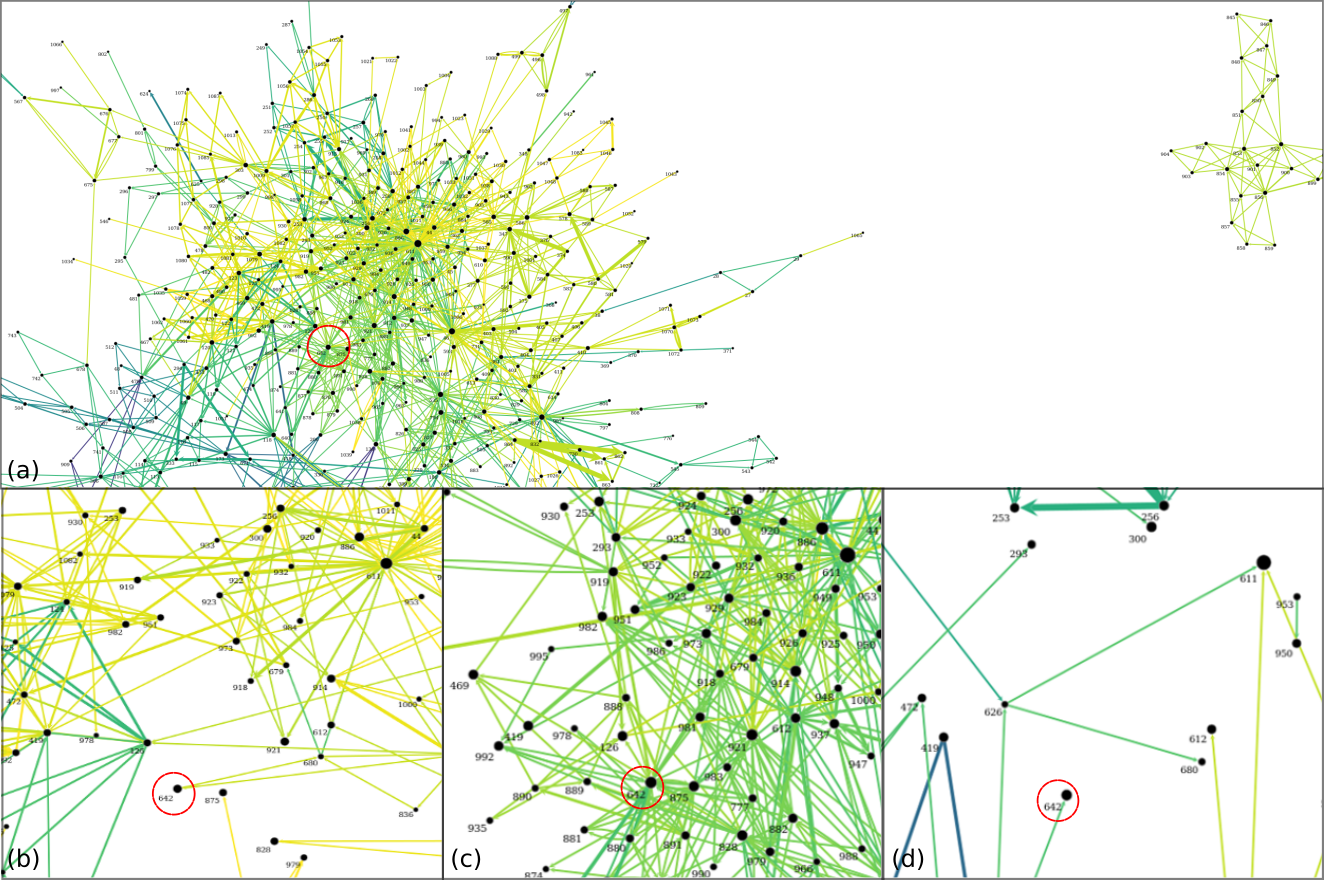
\includegraphics[width=\textwidth]{images/evolution.png}
  \small{
    \caption{\label{fig:evolution}
      At the top (a) is half of compound yearly actor-actor network.  The three bottom images (b), (c) and (d) are closeup around actor 642 during the quarters of the year. }}
\end{figure*}

\subsection{Coursera's dataset}

We used the PP dataset from Coursera 2017 to investigate the construction of a collective activity indicator with \gls{sna} techniques.  We came up with the sociogram (Figure~\ref{fig:evolution}) illustrating an actor-actor dynamics.  Nodes are all learners.  We removed the tutors and the course's mentors to approach Dillenbourg's collaboration definition that we gave in Section~\ref{section:2}.  The users are linked based on their proximity to the previous-3 actors who published in the same discussion.  The arrows' width depend on the messages' timestamp closeness, \# of co-occurrences of the authors and the number of votes that the message collected.  We colored them by discussion, and order them by age, the oldest been the lightest.  This is an intermediate visualization that is used for analysis purposes and will not be presented to the end users for two reasons:
\begin{inparaenum}[\itshape a\upshape)]
\item it gives abstruse information for someone that does not have access to the raw data,
\item it represents the actors as nodes and as we noted in section~\ref{section:3}, we would rather have visualizations showing topics than persons.
\end{inparaenum}
We present it to illustrate what a social network from our dataset looks like, and because, zoomed and reduced to the three snapshots (b), (c), (d), representing three successive yearly quarters, we distinguish an evolving pattern.  In particular a detailed analysis of actor 642, circled in red, show that he started to designate two other messages probably because they were meaningful to him (a), then he engaged in several message exchanges designating others' message meaningful as his where also bringing attention (c), and in the most recent quarter someone commented one of his earlier message (d).  It is not clear from the Figure~\ref{fig:evolution} if actor 642 was part of cycles.  Testing our hypothesis that actors in cycles share a collective dynamic is in our perspectives.

\section{Perspectives and Conclusion}
\label{section:6}


\subsection{Perspectives}

The three test and visualizations presented are preparing further work to build:
\begin{inparaenum}[\itshape a\upshape)]
\item a collective activity indicator taking in account the social network structure, the content of messages and their evolution in time,
\item visualizations for that indicator.
\end{inparaenum}

To further our effort to find visual modalities for the indicator, we conducted a small survey in July 2018 with a 48 tutors from the \gls{vuci} to introduce our project and start engaging them in a co-construction process.   27 were not satisfied or unsure about their current tools' effectiveness to monitor their students' work.  39 agreed or strongly agreed that ICTs could help their students better collaborate and 40 that collaboration was, indeed important for learning.  In a second survey, we plan to ask the tutors the kind of visual representation they would find useful to monitor the collective activities of their students, but also what dimensions of the relationships between messages they would like to leverage to explicit visually those relationships.  This is part of a co-construction approach that should engage the tutors, facilitating its adoption of our visualization while increasing its usability and impact.

Concerning the portability and validation of our pipeline stages (Figure~\ref{fig:pipeline}),  we will need to continue working with several datasets, extending our unified model to incorporate \gls{sna} and \gls{nlp} statistics for all datasets. The portability assumption rests on our capacity to extract periodically, every few minutes, hours or days, data from a main \gls{lms}.  Furthermore, we  will necessitate proper APIs authorizations to make our \gls{ldb} communicate effectively with the \gls{lms}.

%In the experiment with \gls{vuci}, we will certainly run into difficulties to process the \gls{vuci} content dataset because Ivorian french is not standard french and we will not be able to use, as is, common \gls{nlp} tools such as grammar parsers from Python's Nltk library.  But we hope to get promising feedback from the tutors about the usefulness of our prototype to monitor the collective actions of their students.

\subsection{Conclusion}
In this paper, we presented a model to detect collective activities from the forums' discussions.  We based our model on an implicit message relationship and an external parameter set by an observer to explicit that relationship.  Doing so we should facilitating the portability of our indicator to courses covering different domains, spanning various time periods and having different populations. % For example, we suppose that an observer would only have to set his time requirement higher to observe interesting collective dynamics in a short course and set it lower if the course took several months.
\gls{la} is at a turning point where lots of attention is moving to support tools rather than fully automated learning solutions \citep{Kone2018,Baker2016}.
Therefore, we started investigating ways to give a visual feed of the collective dynamics spurring from the \glspl{lms} forums, back to the tutors.  We illustrated with three visualizations our work in progress pushing for more data analysis and data visualization for learning.  We further hope that this work will help tutors and, eventually, students  discover the topic-topic dynamics in their \glspl{mooc} and support collectives activities, so beneficial to learning.

\vfill 

\bibliographystyle{apalike}

\small{\bibliography{bib-csedu19}}

\vfill
\end{document}
